\scanpage{28}
b) Contexte des familles finies de modules quadratiques : $=$ formule, avec $=$ \unsure{démonstration|démonstrati.}

c) \diagram{\begin{tikzcd}[ampersand replacement=\&]
\deleted{I}J \arrow[r,"p"] \& I
\end{tikzcd}}
application \inserted{(surjection si on veut)} d'ens \deleted{\unsure{C|f}}finis,
\[
 I^{-}=\{i\in I\mid\operatorname{Card}p^{-1}(i)\ \text{impair}\}.
\]
\deleted{Je dis que} [p. ex $J$ ens avec relation d'équivalence \inserted{$\mathcal R$}, et $I=J/\mathcal R$]. \deleted{\unsure{O}}Alors
\[
 \omega_J\simeq\omega_{I^{-}}\wedge\bigwedge_{i\in I}\omega_{J_{\unsure{2|i}}}
\]
% slanted, descending toward the right edge; fragmentary traces
\margin{\illegible{1}}

\uline{Compatibilités} entre les isom can. a) b) c)

\figure{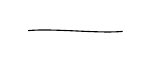
\begin{tikzpicture}
\draw (0,0) .. controls (.32,.03) and (.92,-.04) .. (1.2,-.01);
\end{tikzpicture}}

\uline{Cas d'extensions}
\[
 \{0\}=\deleted{\unsure{0}}E_0\subset E_1\subset E_2\ \mathinner{\cdotp\cdotp}\ \subset E_d=E
\]
\deleted{\unsure{On}} Définir un isom. canonique
\[
 \omega_E\simeq\bigwedge_{1\leq i\leq d}\omega_{E_i/E_{i-1}}
\]
\figure{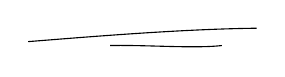
\begin{tikzpicture}
\draw (0,0) .. controls (.76,.06) and (1.95,.16) .. (2.90,.17);
\draw (1.04,-.05) .. controls (1.50,-.04) and (2.10,-.09) .. (2.46,-.05);
\end{tikzpicture}}
% archive sheet number: 27
